%% Submissions for peer-review must enable line-numbering
%% using the lineno option in the \documentclass command.
%%
%% Preprints and camera-ready submissions do not need
%% line numbers, and should have this option removed.
%%
%% Please note that the line numbering option requires
%% version 1.1 or newer of the wlpeerj.cls file, and
%% the corresponding author info requires v1.2

\documentclass[fleqn,10pt,lineno]{wlpeerj} % for journal submissions

% ZNK -- Adding headers for pandoc

\setlength{\emergencystretch}{3em}
\usepackage[unicode=true]{hyperref}


% tightlist command for lists without linebreak
\providecommand{\tightlist}{%
  \setlength{\itemsep}{0pt}\setlength{\parskip}{0pt}}



\usepackage{csquotes}
\usepackage{booktabs}
\usepackage{longtable}
\usepackage{array}
\usepackage{multirow}
\usepackage{wrapfig}
\usepackage{float}
\usepackage{colortbl}
\usepackage{pdflscape}
\usepackage{tabu}
\usepackage{threeparttable}
\usepackage{threeparttablex}
\usepackage[normalem]{ulem}
\usepackage{makecell}
\usepackage{booktabs}
\usepackage{longtable}
\usepackage{array}
\usepackage{multirow}
\usepackage{wrapfig}
\usepackage{float}
\usepackage{colortbl}
\usepackage{pdflscape}
\usepackage{tabu}
\usepackage{threeparttable}
\usepackage{threeparttablex}
\usepackage[normalem]{ulem}
\usepackage{makecell}
\usepackage{xcolor}

\title{Linking watershed nutrient loading to estuary water quality with
Generalized Additive Models}

\author[1]{Michael Schramm}

\corrauthor[1]{Michael
Schramm}{\href{mailto:michael.schramm@ag.tamu.edu}{\nolinkurl{michael.schramm@ag.tamu.edu}}}

\affil[1]{Texas Water Resources Institute, Texas A\&M AgriLife Research,
College Station, Texas, United States}


%
% \author[1]{First Author}
% \author[2]{Second Author}
% \affil[1]{Address of first author}
% \affil[2]{Address of second author}
% \corrauthor[1]{First Author}{f.author@email.com}

% 
\usepackage[style=apa,]{biblatex}
\addbibresource{bibliography.bib}

\begin{abstract}
Evaluating estuary water quality responses to reductions (or increases)
in nutrient loading attributed to on the ground management actions can
be challenging due to the strong influence of environmental drivers on
nutrient loads and non-linear relationships. This study applied
generalized additive models to calculate watershed nutrient loads and
assess responses in estuary water quality to seasonally-adjusted
freshwater inflow and flow-adjusted nutrient loads in Lavaca Bay, Texas.
Lavaca Bay is a secondary embayment on the Texas coast displaying early
potential for eutrophication and water quality degradation. Use of
flow-adjusted nutrient loads allowed the study to evaluate the response
in water quality to changes in nutrient loads driven by anthropogenic
sources. Cross-validation indicated that, despite data constraints,
semiparametric models performed well at nutrient load prediction. Based
on these models, delivered annual nutrient loads varied substantially
from year to year. In contrast, minimal changes in flow-normalized loads
indicate that nutrient loadings were driven by natural variation in
precipitation and runoff as opposed to changes in management of nonpoint
sources. Models indicated no evidence of long-term changes in dissolved
oxygen or chlorophyll-\emph{a} within Lavaca Bay. However, site specific
long-term increases in both organic and inorganic nitrogen are
concerning for their potential to fuel eutrophication. Further analysis
found freshwater inflow had strong influences on nutrient and
chlorophyll-\emph{a} concentrations but there was no evidence that
changes in watershed nutrient loading explained additional variation in
dissolved oxygen and limited evidence that watershed nutrient loadings
explained chlorophyll-\emph{a} concentrations. In addition to providing
a baseline assessment of watershed nutrient loading and water quality
responses in the Lavaca Bay watershed, this study provides
methodological support for the use of semiparametric models in load
regression models and estuary assessments.
% Dummy abstract text. Dummy abstract text. Dummy abstract text. Dummy abstract text. Dummy abstract text. Dummy abstract text. Dummy abstract text. Dummy abstract text. Dummy abstract text. Dummy abstract text. Dummy abstract text.
\end{abstract}

\begin{document}



\flushbottom
\maketitle
\thispagestyle{empty}

\hypertarget{introduction}{%
\section*{Introduction}\label{introduction}}
\addcontentsline{toc}{section}{Introduction}

Similar to many coastal areas globally, the coastal watersheds along the
Texas Gulf coast are facing pressures from growing populations,
increases in point source and non-point source pollution and alterations
to freshwater flows that degrade water quality in downstream estuaries
\autocite{bricker_effects_2008,kennicuttWaterQualityGulf2017,bugica_water_2020}.
Despite these escalating pressures, national scale assessments have
classified coastal estuaries in Texas as moderate or low risk for
eutrophic conditions \autocite{bricker_effects_2008}. However, a suite
of recent studies indicates that estuary water quality dynamics in both
agricultural and urban dominated watersheds within Texas are expressing
conditions that are increasingly conducive to algal blooms and
eutrophication
\autocite{wetzWaterQualityDynamics2016,wetz_exceptionally_2017,bugica_water_2020,chinPhytoplanktonBiomassCommunity2022}.
With identification of several localized areas of estuary water quality
concern along the Texas coast \autocite{bugica_water_2020}, localized
studies are being prioritized to better inform management actions.

The goal of this project is to assess watershed nutrient loading and the
resulting water quality responses in Lavaca Bay, Texas. Lavaca Bay is a
secondary bay in the larger Matagorda Bay system located roughly halfway
between Houston, Texas and Corpus Christi, Texas. Lavaca Bay faces
substantial challenges associated with legacy contamination but general
water quality parameters such as dissolved oxygen (DO), nutrients, and
biological parameters have been well within state water quality
standards. Despite largely meeting state designated water quality
thresholds, there have been concerning declines in abundance, biomass,
and diversity of benthic fauna in Lavaca Bay
\autocite{beserespollackLongtermTrendsResponse2011}. These declines are
partially attributed to reductions in freshwater inflow and changes in
estuary salinity and are indicative of an already stressed system
\autocite{beserespollackLongtermTrendsResponse2011,palmerImpactsDroughtsLow2015,montagnaAssessmentRelationshipFreshwater2020}.
More recently, significant linear increases in total phosphorus (TP),
orthophosphate, total Kjeldahl nitrogen (TKN), and chlorophyll-\emph{a}
concentrations were identified at monitoring sites within Lavaca Bay
\autocite{bugica_water_2020}. While significant nitrogen increases were
only identified in TKN, both organic and inorganic forms of nitrogen can
serve as potential indicators of eutrophication status and estuary
health \autocite{jessenMarineEutrophication2015}. Nitrogen is generally
considered the limiting factor for primary production in many Texas
estuaries
\autocite{gardnerNitrogenFixationDissimilatory2006,houTransformationFateNitrate2012,doradoUnderstandingInteractionsFreshwater2015,paudelRelationshipSuspendedSolids2019,wetz_exceptionally_2017}.
However, estuaries can display nitrogen and phosphorus co-limitation
that may vary temporally and spatially
\autocite{elserGlobalAnalysisNitrogen2007,conleyControllingEutrophicationNitrogen2009},
emphasizing a need to assess a variety of nutrient species.

There are ongoing efforts between local, state, and federal agencies to
address water quality impairments in the freshwater portions of the
Lavaca Bay watershed
\autocite{jainTechnicalSupportDocument2021,schrammLavacaRiverWatershed2018,bertholdDirectMailingEducation2021}.
However, on a statewide scale, these approaches have shown limited
success and emphasize a need for improved methods to assess and link
management actions with downstream water quality
\autocite{schrammTotalMaximumDaily2022}. Such methods could help
identify and replicate effective water quality management actions across
the state . The identification and communication of changes and trends
in water quality is complicated by the fact that trends are often
non-linear and confounded by precipitation and runoff that hinder
traditional analysis
\autocite{wazniakLinkingWaterQuality2007,lloydMethodsDetectingChange2014}.
The development and application of flexible statistical methods such as
Weighted Regressions on Time, Discharge and Season
\autocite[WRTDS,][]{hirschWeightedRegressionsTime2010} and Generalized
Additive Models \autocite[GAMs,][]{woodFastStableRestricted2011} have
provided effective tools for researchers to quantify and communicate
non-linear changes in river and estuary pollutant loadings.

WRTDS calculates a time series of in-stream concentrations or loads
(daily, monthly, or annually) and flow-normalized estimates of
concentrations and loads using locally weighted regression for unique
combinations of time, discharge, and season. WRTDS has been widely used
to assess and identify trends in riverine nutrients
\autocite{oelsner_recent_2019,stackpooleLongTermMississippi2021},
chlorides \autocite{stetsIncreasingChlorideRivers2018}, and other
pollutants of concern \autocite{shodaWaterqualityTrendsRivers2019}.
WRTDS has also been successfully adapted to assess trends in estuary
water quality concentrations \autocite{beckFourDecadesWater2018}.

While WRTDS is a statistical approach developed specifically for water
quality applications, GAMs are a broadly applicable statistical method.
GAMs are a semiparametric extension of generalized linear models where
the response variable is modeled as the sum of multiple unknown smooth
functions and parametric linear predictors
\autocite{woodFastStableRestricted2011}. Although the underlying
parameter estimation procedure of GAMs are substantially different than
WRTDS, both the functional form and results have been demonstrated to be
similar when assessing nutrient concentration trends
\autocite{beckNumericalQualitativeContrasts2017}. Water quality
applications of GAMs have included river and catchment nutrient
concentration and load estimation
\autocite{wangLoadEstimationUncertainties2011,kroonRiverLoadsSuspended2012,kuhnertQuantifyingTotalSuspended2012,robson_prediction_2015-1,hagemannEstimatingNutrientOrganic2016,mcdowell_implications_2021,biagi_novel_2022},
and assessment of temporal trends of nutrients
\autocite{beckNumericalQualitativeContrasts2017,murphyGeneralizedAdditiveModel2019},
phytoplankton \autocite{bergbuschUnexpectedShiftPhytoplankton2021}, and
cyanobacteria \autocite{hayesEffectsLakeWarming2020}. Recently GAMs have
also been used to link water quality responses in receiving water bodies
to changes in nonpoint source nutrient inputs
\autocite{murphyNutrientImprovementsChesapeake2022}. For a substantial
discussion on the differences (and similarities) between GAMs and WRTDS
for water quality applications readers are referred to
\textcite{beckNumericalQualitativeContrasts2017}.

To provide actionable information for resource managers in Lavaca Bay,
water quality conditions must be evaluated relative to changes in
natural environmental drivers to better understand and manage potential
human impacts. This study utilizes GAMs to develop estimates of
delivered and flow-normalized nutrient loads and assess estuary water
quality responses to changes in loads delivered to Lavaca Bay. GAMs were
chosen over other regression-based approached for use in this study due
to; (1) the ability to easily explore and incorporate different model
terms; (2) the incorporation of non-linear smooth functions that do not
require explicit a priori knowledge of the expected shape; and (3)
inclusion of a link function that related the expected value of the
response to linear predictors thus avoiding unneeded data
transformations and bias corrections. The exploratory study also
assesses the response of water quality parameters in Lavaca Bay over
time and in response to freshwater inflow controlled for seasonality and
to watershed nutrient loads that are controlled for environmentally
driven variation.

\hypertarget{methods-and-materials}{%
\section*{Methods and Materials}\label{methods-and-materials}}
\addcontentsline{toc}{section}{Methods and Materials}

\hypertarget{location-and-data}{%
\subsection*{Location and Data}\label{location-and-data}}
\addcontentsline{toc}{subsection}{Location and Data}

Lavaca Bay is a 190 km\textsuperscript{2} estuary with the majority of
freshwater inflow provided by the Lavaca and Navidad River systems
(Fig.~\ref{fig:fig1}). Lavaca Bay is relatively shallow with an average
depth of 1.2 m and a generally well mixed and turbid water column
\autocite{beserespollackLongtermTrendsResponse2011,montagnaAssessmentRelationshipFreshwater2020}.
The Garcitas-Arenosa, Placedo Creek, and Cox Bay subwatersheds provide
additional freshwater inflows. The proximity to freshwater inputs in the
upper Lavaca Bay results in a strong mean salinity and variance gradient
\autocite{montagnaAssessmentRelationshipFreshwater2020}. Average
salinity ranges from 12 psu near the Lavaca River mouth to 23 psu at the
mouth of Lavaca Bay. The variance is inversely correlated with mean
salinity. The entire watershed area is 8,149 km\textsuperscript{2} and
primarily rural. Watershed land cover and land use is 50\% grazed
pasture and rangeland, 20\% cultivated cropland (primarily rows crops
such as corn, cotton, and sorghum), and 5\% suburban/urban. Pasture and
rangeland is concentrated in the Lavaca River watershed, while
cultivated crops are generally located along the eastern tributaries of
the Navidad river. The Lavaca and Navidad River watersheds are a
combined 5,966 km\textsuperscript{2}, or approximately 73\% of the
entire Lavaca Bay watershed area. Discharge from the Navidad River is
regulated by Lake Texana which has been in operation since 1980. Lake
Texana provides 0.210 km\textsuperscript{3} of water storage and
discharges into the tidal section of the Navidad River which ultimately
joins the tidal section of the Lavaca River 15 km upstream of the
confluence with the Lavaca Bay.

\begin{figure}

{\centering 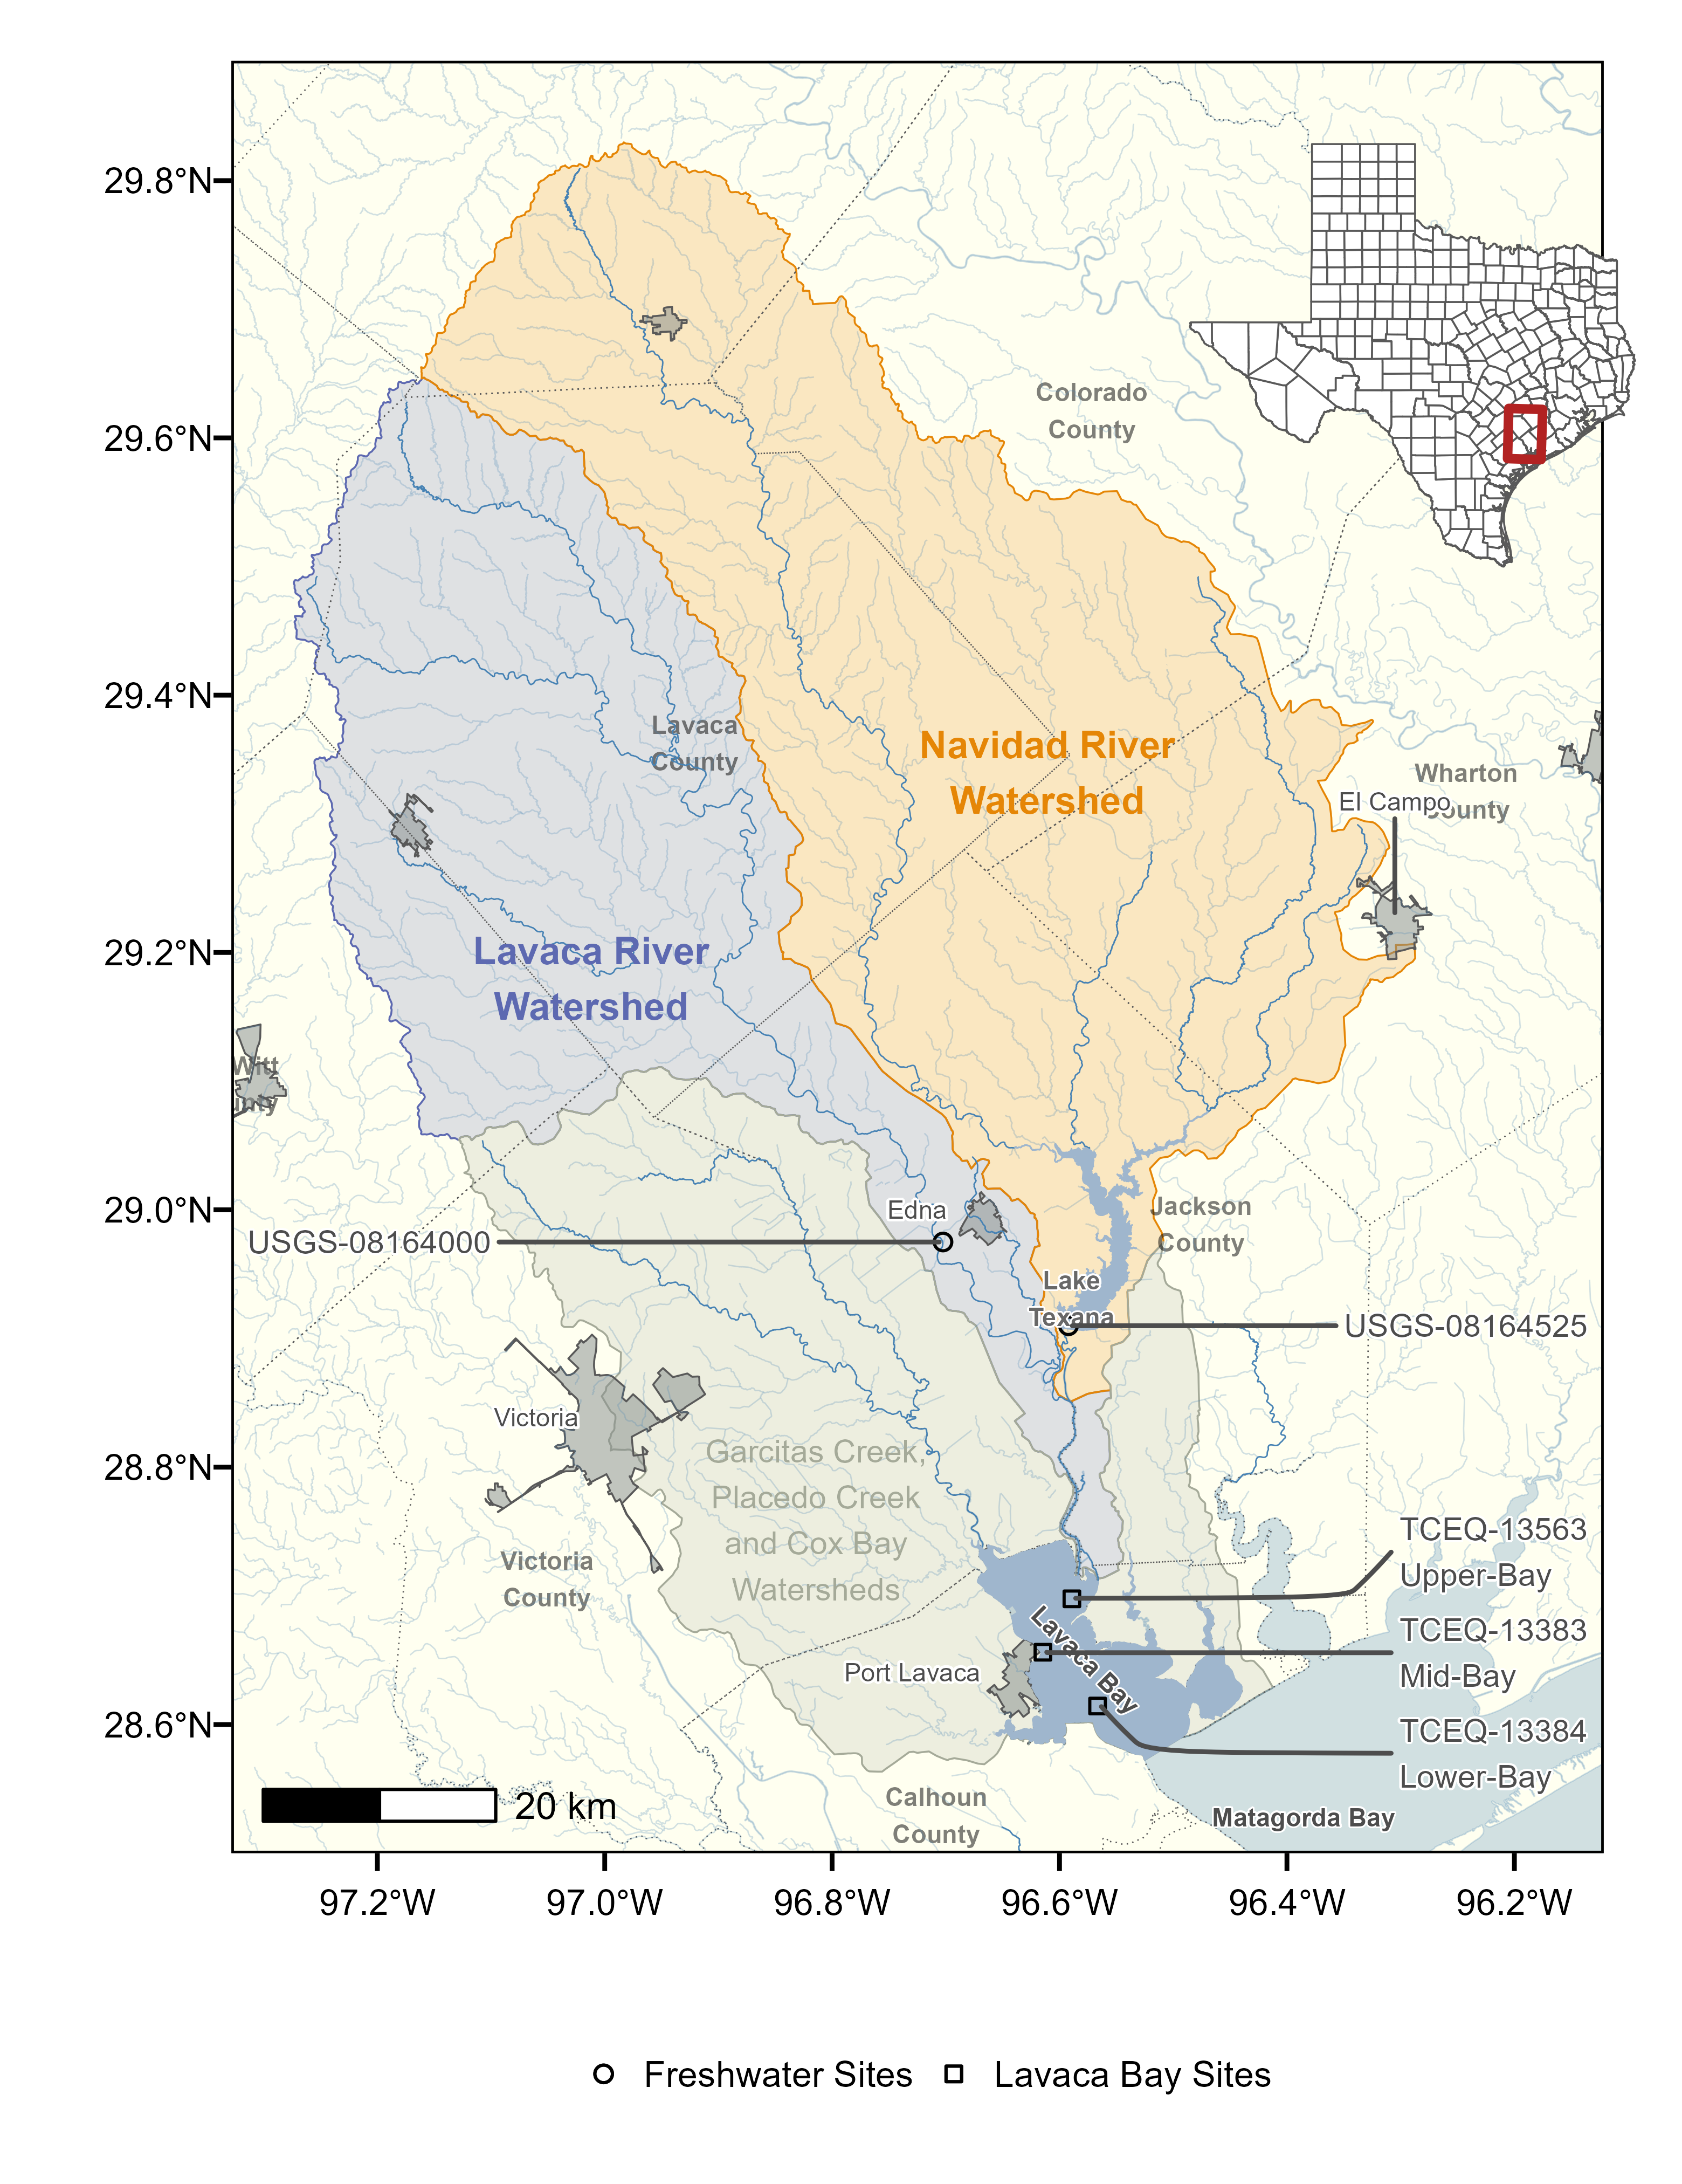
\includegraphics[width=5.2in,]{Schramm-2023-08-PeerJ_files/figure-latex/fig1} 

}

\caption{Map of Lavaca Bay watershed. The freshwater sites are the most downstream freshwater stream locations with water quality and streamflow data used for nutrient load models. Water quality concentration data at the three Lavaca Bay sites were used to assess relationships between freshwater flows, loads and estuary water quality.}\label{fig:fig1}
\end{figure}

Daily discharges for the Lavaca River (USGS-08164000,
Fig.~\ref{fig:fig1}) were obtained from the United States Geologic
Survey (USGS) National Water Information System
(\url{https://waterdata.usgs.gov/nwis}) using the \emph{dataRetrieval} R
package \autocite{deciccoDataRetrievalPackagesDiscovering2022}. Gaged
daily discharges from the outlet of Lake Texana on the Navidad River
(USGS-0816425) were provided by the Texas Water Development Board (TWDB)
(April 21, 2022 email from R. Neupane, TWDB).

Water quality data for the two freshwater and three estuary locations
were obtained from the Texas Commission on Environmental Quality (TCEQ)
Surface Water Quality Monitoring Information System. Data submitted
through the system are required to be collected under Quality Assurance
Project Plans and lab method procedures outlined by the TCEQ's
procedures manual. These operating procedures ensure consistent
collection and laboratory methods are applied between samples collected
by different entities and under different projects. All sites had
varying time periods and availability of water quality data. For
freshwater locations, TP from January 2000 through December 2020 and
nitrate-nitrogen (NO\textsubscript{3}) data from January 2005 through
December 2020 were downloaded (Table~\ref{tab:table1}). Less than
5-years of total nitrogen and TKN concentration data were available at
the freshwater sites and deemed insufficient to develop load estimation
models
\autocite{horowitzEvaluationSedimentRating2003,snelderEstimationCatchmentNutrient2017}.
The three estuary sites included an upper-bay site near the outlet of
the Lavaca River system (TCEQ-13563), a mid-bay site (TCEQ-13383), and
the lower-bay site near the mouth of the Bay (TCEQ-13384). For estuary
locations, we obtained data for TP, Nitrite+Nitrate
(NO\textsubscript{\emph{X}}), TKN, chlorophyll-\emph{a}, and DO
concentrations from January 2005 through December 2020
(Table~\ref{tab:table2}). Freshwater nutrient samples were collect 0.3
meters below the surface or halfway between the surface and bottom if
depth was insufficient. Estuary nutrient samples were all collected 0.3
meters below the surface. Estuary DO measurements were made at 3
locations along the water column (0.3 meters, mid-depth, and bottom) and
averaged. All water quality data was collected approximately quarterly.

\begin{table}

\caption{\label{tab:table1}Summary of gauged streamflow and freshwater water quality samples between January 1, 2000 and December 31, 2020.}
\centering
\begin{threeparttable}
\begin{tabular}[t]{>{\raggedright\arraybackslash}p{2.5cm}>{\raggedright\arraybackslash}p{2.5cm}llllrr}
\toprule
Station ID and Watershed & Parameter & Mean & SD & N & Method & AWRL\textsuperscript{a} & Criteria\textsuperscript{b}\\
\midrule
 & TP (mg/L) & 0.21 & 0.09 & 80 & EPA 365.1 & 0.06 & 0.69\\

 & NO\textsubscript{3} (mg/L) & 0.18 & 0.24 & 74 & EPA 353.2 & 0.05 & 1.95\\

\multirow{-3}{2.5cm}{\raggedright\arraybackslash USGS-08164000, Lavaca River} & Mean Daily Streamflow (cfs) & 332.78 & 1667.47 & 7671 &  &  & \\
\cmidrule{1-8}
 & TP (mg/L) & 0.20 & 0.08 & 81 & EPA 365.1 & 0.06 & 0.20\\

 & NO\textsubscript{3} (mg/L) & 0.29 & 0.26 & 62 & EPA 353.2 & 0.05 & 0.37\\

\multirow{-3}{2.5cm}{\raggedright\arraybackslash USGS-08164525, Navidad River} & Mean Daily Streamflow (cfs) & 666.14 & 2957.79 & 7671 &  &  & \\
\bottomrule
\end{tabular}
\begin{tablenotes}
\item[a] Ambient water reporting limit (AWRL) represents the highest concentration that can be used as a reporting limit by a laboratory for inclusion in the state's monitoring data.
\item[b] The state of Texas has not adopted numeric criteria for nutrients, these criteria represent screening levels used by the state for assessment purposes.
\end{tablenotes}
\end{threeparttable}
\end{table}

\begin{table}

\caption{\label{tab:table2}Summary of estuary water quality samples collected between January 1, 2005 and December 31, 2020.}
\centering
\begin{threeparttable}
\begin{tabular}[t]{>{\raggedright\arraybackslash}p{2cm}llll>{\raggedright\arraybackslash}p{2.5cm}rr}
\toprule
Station ID & Parameter & Mean & SD & N & Method & AWRL\textsuperscript{a} & Criteria\textsuperscript{b}\\
\midrule
 & TP (mg/L) & 0.13 & 0.06 & 50 & EPA 365.1 & 0.06 & 0.21\\

 & NO\textsubscript{x} (mg/L) & 0.09 & 0.13 & 53 & EPA 353.2 & 0.05 & \\

 & TKN (mg/L) & 0.94 & 0.37 & 49 & EPA 351.2 & 0.20 & \\

 & Chlorophyll-\textit{a} (ug/L) & 9.67 & 5.33 & 49 & EPA 445.0 & 3.00 & 11.60\\

\multirow{-5}{2cm}{\raggedright\arraybackslash TCEQ-13563, Upper-Bay} & DO (mg/L) & 7.91 & 1.34 & 56 & ASTM D888-09(C) and TCEQ SOP V1 &  & 5.00\\
\cmidrule{1-8}
 & TP (mg/L) & 0.11 & 0.05 & 47 & EPA 365.1 & 0.06 & 0.21\\

 & NO\textsubscript{x} (mg/L) & 0.07 & 0.15 & 51 & EPA 353.2 & 0.05 & \\

 & TKN (mg/L) & 0.94 & 0.49 & 45 & EPA 351.2 & 0.20 & \\

 & Chlorophyll-\textit{a} (ug/L) & 9.43 & 5.31 & 47 & EPA 445.0 & 3.00 & 11.60\\

\multirow{-5}{2cm}{\raggedright\arraybackslash TCEQ-13383, Mid-Bay} & DO (mg/L) & 7.22 & 1.35 & 55 & ASTM D888-09(C) and TCEQ SOP V1 &  & 5.00\\
\cmidrule{1-8}
 & TP (mg/L) & 0.08 & 0.03 & 51 & EPA 365.1 & 0.06 & 0.21\\

 & NO\textsubscript{x} (mg/L) & 0.06 & 0.08 & 52 & EPA 353.2 & 0.05 & \\

 & TKN (mg/L) & 0.76 & 0.40 & 48 & EPA 351.2 & 0.20 & \\

 & Chlorophyll-\textit{a} (ug/L) & 8.22 & 6.44 & 46 & EPA 445.0 & 3.00 & 11.60\\

\multirow{-5}{2cm}{\raggedright\arraybackslash TCEQ-13384, Lower-Bay} & DO (mg/L) & 7.51 & 1.32 & 54 & ASTM D888-09(C) and TCEQ SOP V1 &  & 5.00\\
\bottomrule
\end{tabular}
\begin{tablenotes}
\item[a] Ambient water reporting limit (AWRL) represents the highest concentration that can be used as a reporting limit by a laboratory for inclusion in the state's monitoring data.
\item[b] The state of Texas has not adopted numeric criteria for nutrients, these criteria represent screening levels used by the state for assessment purposes. NO\textsubscript{x} and TKN parameters are not currently screened by the state and do not have an associated screening level.
\end{tablenotes}
\end{threeparttable}
\end{table}

\hypertarget{estimating-watershed-based-nutrient-loads}{%
\subsection*{Estimating Watershed Based Nutrient
Loads}\label{estimating-watershed-based-nutrient-loads}}
\addcontentsline{toc}{subsection}{Estimating Watershed Based Nutrient
Loads}

Estimates of NO\textsubscript{3} and TP loads at the Lavaca River
(USGS-08164000) and the outlet of Lake Texana on the Navidad River
(USGS-08164525) were developed using GAMs relating nutrient
concentration to river discharge, season, and time. Separate models were
fit at each station for each parameter and used to predict nutrient
concentrations for each day in the study period. GAMs were fit using the
\emph{mgcv} package in R which makes available multiple types of smooth
functions with automatic smoothness selection
\autocite{woodFastStableRestricted2011}. The general form of the model
related NO\textsubscript{3} or TP concentration to a long term trend,
season, streamflow, and two different antecedent discharge terms, shown
in Eq. \ref{eq1}:

\begin{align}
g(\mu) &= \alpha + f_1(ddate) + f_2(yday) + f_3(log(1+Q)) + f_4(ma) + f_5(fa), \nonumber \\
y &\sim \mathcal{N}(\mu,\,\sigma^{2})
\label{eq1}
\end{align}

where \(\mu\) is the conditional expected NO\textsubscript{3} or TP
concentration, \(g()\) is the log-link, \(\alpha\) is the intercept,
\(f_n()\) are smoothing functions. \(y\) is the response variable
(NO\textsubscript{3} or TP concentration) modeled as normally
distributed with mean \(\mu\) and standard deviation \(\sigma\).
\emph{ddate} is the date converted to decimal notation, \emph{yday} is
numeric day of year (1-366), and \emph{Q} is the mean daily streamflow.

Moving average (\emph{ma}) is an exponentially smoothed moving average
that attempts to incorporate the influence of prior streamflow events on
concentration at the current time period
\autocite{wangLoadEstimationUncertainties2011,kuhnertQuantifyingTotalSuspended2012,wangSedimentConcentrationPrediction2013a,zhang_improving_2017},
using Eq. \ref{eq2}:

\begin{equation}
ma(d) = \frac{Q_j + dQ_{j-1} + \mathellipsis + d^{j-1}Q_1}{1+d+...+d^{j-1}}
\label{eq2}
\end{equation}

where \emph{ma} at discount factor \emph{d} is calculated using flows
\((Q_1,Q_2,...,Q_j)\) for days 1 through \emph{j}. Here, as \emph{d}
approaches zero, the time series becomes the daily observed values and
as \emph{d} gets closer to one, the time series becomes the mean flow.
Although \textcite{kuhnertQuantifyingTotalSuspended2012} and
\textcite{wangSedimentConcentrationPrediction2013a} suggest using
multiple covariates with \emph{d} set at different values from 0.75 to
0.99, \textcite{robson_prediction_2015-1} and
\textcite{zhang_improving_2017} found substantial improvements in
statistical nutrient models with \emph{d} equal to 0.95 which was
adopted in this study.

Flow anomaly (\emph{fa}) is a dimensionless term that represents how wet
or dry (or how anomalous) the current time period is from previous time
periods
\autocite{vecchiaTrendsConcentrationsUse2009,zhang_improving_2017}.
Long-term flow anomaly (\emph{ltfa}) is the streamflow over the previous
year relative to the entire period
\autocite[Eq.~\ref{eq3},][]{zhang_improving_2017} and and the short-term
flow anomaly (\emph{stfa}) calculated as the current day flow compared
to the preceding 1-month streamflow
\autocite[Eq.~\ref{eq4},][]{zhang_improving_2017}:

\begin{align}
ltfa(t) &= \bar{x}_{1\,year}(t) - \bar{x}_{entire\,period}, \label{eq3}\\
stfa(t) &= x_{current\,day}(t) - \bar{x}_{1\,month}(t) \label{eq4}
\end{align}

where \(x\) are the averages of log-transformed streamflow over the
antecedent period (\emph{1-year}, \emph{1-month}, etc.) for time
\emph{t}. We used \emph{ltfa} in NO\textsubscript{3} models and
\emph{stfa} in TP models based on previous work demonstrating major
improvements in NO\textsubscript{\emph{X}} regression models that
incorporated \emph{ltfa} and moderate improvements in TP regression
models that incorporated \emph{stfa} \autocite{zhang_improving_2017}.
Moving averages and flow anomalies were calculated with the \emph{adc} R
package \autocite{schrammAdcCalculateAntecedant2023}.

The calculation of model terms for the Lake Texana site were modified
because daily loads are not a function of natural stream flow processes
alone, but of dam releases and nutrient concentrations at the discharge
point of the lake. \emph{Q}, \emph{ma}, and \emph{fa} terms were
calculated based on total gaged inflow from the 4 major tributaries to
the lake. Thin-plate regression splines were used for \emph{ddate},
\emph{log(1+Q)}, \emph{fa}, and \emph{ma}. A cyclic cubic regression
spline was used for \emph{yday} to ensure the ends of the spline match
(day 1 and day 366 are expected to match). First order penalties were
applied to the smooths of flow-based variables which penalize departures
from a flat function to help constrain extrapolations for high flow
measurements.

Left-censored data were not uncommon in this dataset (4\% of TP samples
and 20\% of NO\textsubscript{3} samples). Several methods are available
to account for censored data. We transformed left-censored nutrient
concentrations to one-half the detection limit. Although this simple
approach can introduce bias
\autocite{hornungEstimationAverageConcentration1990}, we considered it
acceptable because high concentrations and loadings are associated with
high-flow events and low-flow/low-concentration events will account for
a small proportion of total loadings
\autocite{mcdowell_implications_2021}.

Daily loads were estimated as the predicted concentration multiplied by
the daily streamflow. For the Navidad River (USGS-08164525) site, daily
loads at the dam were calculated from the discrete daily concentration
at the discharge point of the lake and corresponding reported daily
discharge from the dam. Flow-normalized loads were estimated similar to
WRTDS by setting flow-based covariates on each day of the year equal to
each of the historical values for that day of the year over the study
period \autocite{hirschWeightedRegressionsTime2010}. The flow-normalized
estimate was calculated as the mean of all the predictions for each day
considering all possible flow values. Standard deviations and 90\%
credible intervals were obtained by drawing samples from the
multivariate normal posterior distribution of the fitted GAM
\autocite{woodConfidenceIntervalsGeneralized2006,marraCoveragePropertiesConfidence2012,mcdowell_implications_2021}.
GAM performance was evaluated with repeated 5-fold cross validation
\autocite{burmanComparativeStudyOrdinary1989} using average
Nash-Sutcliffe Efficiency (NSE), Pearson sample correlation (\emph{r})
and percent bias (PBIAS) metrics.

\hypertarget{linking-estuary-water-quality-to-hydrology-and-nutrient-loads}{%
\subsection*{Linking Estuary Water Quality to Hydrology and Nutrient
Loads}\label{linking-estuary-water-quality-to-hydrology-and-nutrient-loads}}
\addcontentsline{toc}{subsection}{Linking Estuary Water Quality to
Hydrology and Nutrient Loads}

To test if changes in freshwater inflow and nutrient loading had
explanatory effect on changes in estuary water quality a series of GAM
models were fit at each site relating parameter concentration to
temporal trends (Eq.~\ref{eq5}), temporal trends and inflow
(Eq.~\ref{eq6}), and temporal trends, inflow, and nutrient loads
(Eq.~\ref{eq7}): \begin{align}
g(\mu) &= \alpha + f_1(ddate) + f_2(yday), \label{eq5} \\
g(\mu) &= \alpha + f_1(ddate) + f_2(yday) + f_3(Q), \label{eq6} \\
g(\mu) &= \alpha + f_1(ddate) + f_2(yday) + f_3(Q) + f_4(Load) \label{eq7}
\end{align}

where \(\mu\) is the conditional expected response (nutrient
concentration), \(g()\) is the log link, and response variable was
modeled as Gamma distributed with mean \(\mu\) and scale \(\lambda\).
\(f_1(ddate)\) is decimal date smoothed with a thin-plate regression
spline, \(f_2(yday)\) is the numeric day of year smoothed with a cyclic
cubic regression spline. Prior work has shown that many water quality
parameters may have lagged effects lasting days or even months following
storms and large discharge events
\autocite{mooneyWatershedExportEvents2012a,wetzExtremeFutureEstuaries2013,bukaveckasInfluenceStormEvents2020,walkerTimescalesMagnitudeWater2021}.
\textcite{walkerTimescalesMagnitudeWater2021} showed the impact of large
flow events like Hurricane Harvey had somewhat short water quality
impacts in Lavaca Bay and adjacent estuary systems, ranging somewhere
around 20 days to a few months. We incorporate this lag effect by using
cumulative totals for \(f_3(Q)\) and \(f_4(Load)\). \(f_3(Q)\) is the
cumulative of the previous 20 days of inflow (combined measurements from
Lavaca River and Navidad River) and \(f_4(Load)\) is the cumulative of
the previous 20 days total NO\textsubscript{3} or TP watershed load,
both smoothed with thin plate regression splines. The set of models
specified for each water quality response are in Table~\ref{tab:table3}.

\begin{table}

\caption{\label{tab:table3}Set of GAM models specified for each water quality parameter response.}
\centering
\begin{tabular}[t]{lll}
\toprule
Parameter & Model & Model Terms\\
\midrule
 & Temporal & s(ddate) + s(yday)\\

 & Flow & s(ddate) + s(yday) + s(Q)\\

\multirow{-3}{*}{\raggedright\arraybackslash TP} & Flow+Load & s(ddate) + s(yday) + s(Q) + s(TP Load)\\
\cmidrule{1-3}
 & Temporal & s(ddate) + s(yday)\\

 & Flow & s(ddate) + s(yday) + s(Q)\\

\multirow{-3}{*}{\raggedright\arraybackslash NO\textsubscript{x}} & Flow+Load & s(ddate) + s(yday) + s(Q) + s(NO\textsubscript{3} Load)\\
\cmidrule{1-3}
 & Temporal & s(ddate) + s(yday)\\

 & Flow & s(ddate) + s(yday) + s(Q)\\

\multirow{-3}{*}{\raggedright\arraybackslash Chlorophyll-\textit{a}} & Flow+Load & s(ddate) + s(yday) + s(Q) + s(TP Load) + s(NO\textsubscript{3} Load)\\
\cmidrule{1-3}
 & Temporal & s(ddate) + s(yday)\\

 & Flow & s(ddate) + s(yday) + s(Q)\\

\multirow{-3}{*}{\raggedright\arraybackslash Dissolved Oxygen} & Flow+Load & s(ddate) + s(yday) + s(Q) + s(TP Load) + s(NO\textsubscript{3}  Load)\\
\cmidrule{1-3}
 & Temporal & s(ddate) + s(yday)\\

\multirow{-2}{*}{\raggedright\arraybackslash TKN} & Flow & s(ddate) + s(yday) + s(Q)\\
\bottomrule
\end{tabular}
\end{table}

Because streamflow and nutrient loads are tightly correlated, freshwater
inflow can mask signals due to changes in nutrient loads alone.
Following the methodology implemented by
\textcite{murphyNutrientImprovementsChesapeake2022}, both freshwater
inflow and nutrient loads were prepossessed to account for season and
streamflow respectively. Cumulative inflow values were replaced by
seasonally adjusted cumulative inflow obtained from the residuals of a
GAM model fit between season(day of year) and log transformed cumulative
inflow. Nutrient loads utilized the flow-normalized loads estimated in
the previous section.

This study used an information theoretic approach to evaluate evidence
of model covariate effects on Lavaca Bay water quality. Model
probabilities were calculated and compared using the
AIC\textsubscript{c} scores between each group of temporal, inflow, and
inflow+load models \autocite{burnhamAICModelSelection2011}. Improvements
in model probabilities provide evidence that the terms explain
additional variation in the response variable.

\hypertarget{results}{%
\section*{Results}\label{results}}
\addcontentsline{toc}{section}{Results}

\hypertarget{watershed-nutrient-loads}{%
\subsection*{Watershed Nutrient Loads}\label{watershed-nutrient-loads}}
\addcontentsline{toc}{subsection}{Watershed Nutrient Loads}

Predictive performance of nutrient loads ranged from ``satisfactory'' to
``very good'' based on standardized evaluation metrics of NSE, \emph{r},
and PBIAS \autocite{moriasiHydrologicWaterQuality2015} calculated using
5-fold cross validation. Median goodness-of-fit metrics for
NO\textsubscript{3} models in the Lavaca River were 0.34 NSE, 0.70
\emph{r}, and 2.00 PBIAS. Navidad River NO\textsubscript{3} models
appeared to perform slightly better with 0.48 NSE and 0.87 \emph{r} but
with higher bias at 10.90 PBIAS. Generally, TP models performed better
than NO\textsubscript{3} models. Median goodness-of-fit metrics for TP
in the Lavaca River were 0.81 NSE, 0.93 \emph{r}, and -7.20 PBIAS.
Navidad River TP models had similar performance with 0.91 NSE, 0.99
\emph{r}, and -3.30 PBIAS. Density plots of metrics show similar
distribution of values between sites for the same parameter, with the
exception \emph{r} values for NO\textsubscript{3} loads where Lavaca
River had a much larger variance in values compared to the Navidad River
(Fig.~\ref{fig:fig2}). TP GAMS had higher average NSE and \emph{r}
values and lower variance in metric values compared to
NO\textsubscript{3}.

\begin{figure}

{\centering 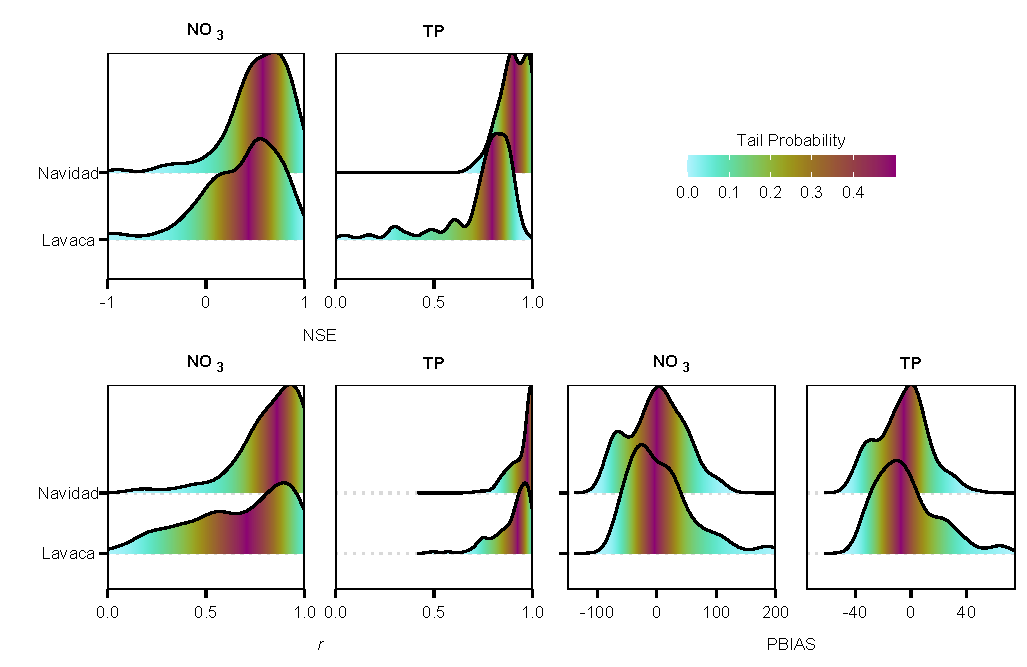
\includegraphics[width=1\linewidth,]{Schramm-2023-08-PeerJ_files/figure-latex/fig2} 

}

\caption{Density plots of goodness-of-fit metrics (NSE, \textit{r}, and PBIAS) from repeated 5-fold cross validation between predicted nutrient loads from GAM models and measured nutrient loads. Color indicates the tail probability calculated from the empirical cumulative distribution of the goodness-of-fit metrics. Values closer to 1 for NSE and r and values closer to 0 for PBIAS represent more ideal goodness-of-fit assessments.}\label{fig:fig2}
\end{figure}

Annual NO\textsubscript{3} and TP loads show considerable variation,
generally following patterns in discharge (Fig.~\ref{fig:fig3}, Fig.
\ref{fig:fig4}). Flow-normalized TP loads at both sites and
flow-normalized NO\textsubscript{3} loads in the Lavaca River indicated
watershed based loads did not change much over time when accounting for
variation driven by streamflow (Fig.~\ref{fig:fig3}). Flow-normalized
loads in the Lavaca River showed small variation over time with some
decreases in NO\textsubscript{3} loads since 2013.

\begin{figure}

{\centering 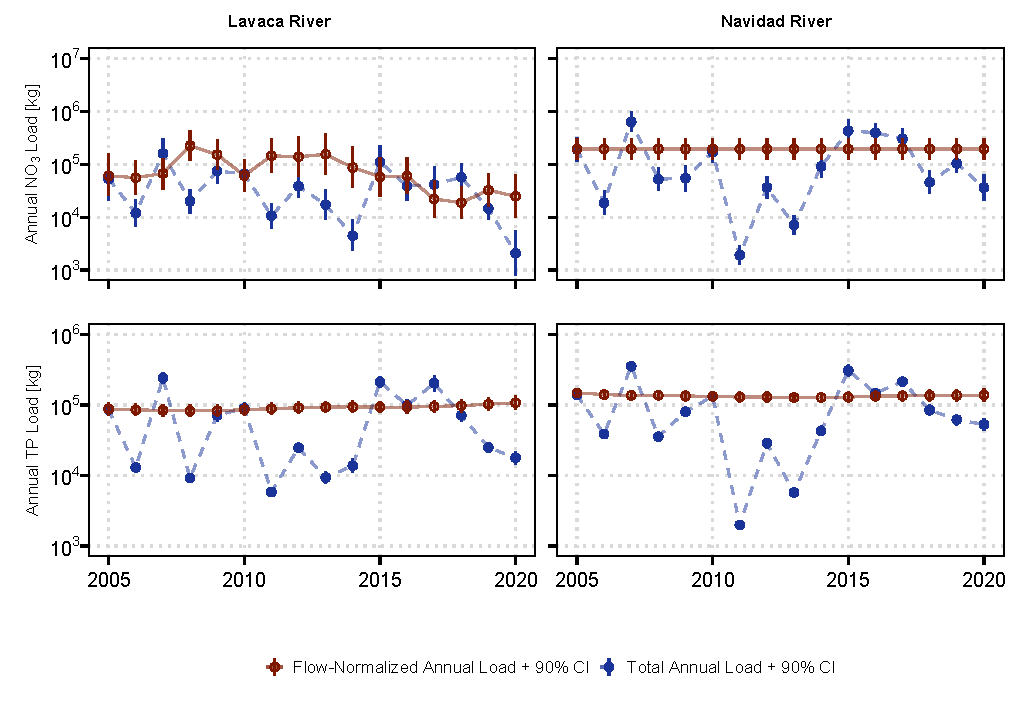
\includegraphics[width=1\linewidth,]{Schramm-2023-08-PeerJ_files/figure-latex/fig3} 

}

\caption{Aggregated estimated annual and flow-normalized annual NO\textsubscript{3} and TP loads for the Lavaca (USGS-08164000) and and Navidad (USGS-08164525) Rivers.}\label{fig:fig3}
\end{figure}

Aggregated across both sites, the mean annual NO\textsubscript{3} load
from 2005 through 2020 was 205,405 kg (126,867 kg - 341,569 kg, 90\%
CI). Annual NO\textsubscript{3} loads ranged from 12,574 kg in 2011 to
794,510 kg in 2007. Total annual TP loads ranged from 7,839 kg in 2011
to 595,075 kg in 2007. Mean annual TP loading from 2005 through 2020 was
182,673 kg (152,227 kg - 219,310 kg, 90\% CI). On average, the Navidad
River accounted for 68\% of NO\textsubscript{3} loads and 59\% of TP
loads from 2005 through 2020. However, during periods of extreme drought
the Lavaca River became the primary source of nutrient loading in the
watershed with the Navidad River only accounting for 15\% and 25\% of
NO\textsubscript{3} and TP loads in 2011 (Fig.~\ref{fig:fig4}).

\begin{figure}

{\centering 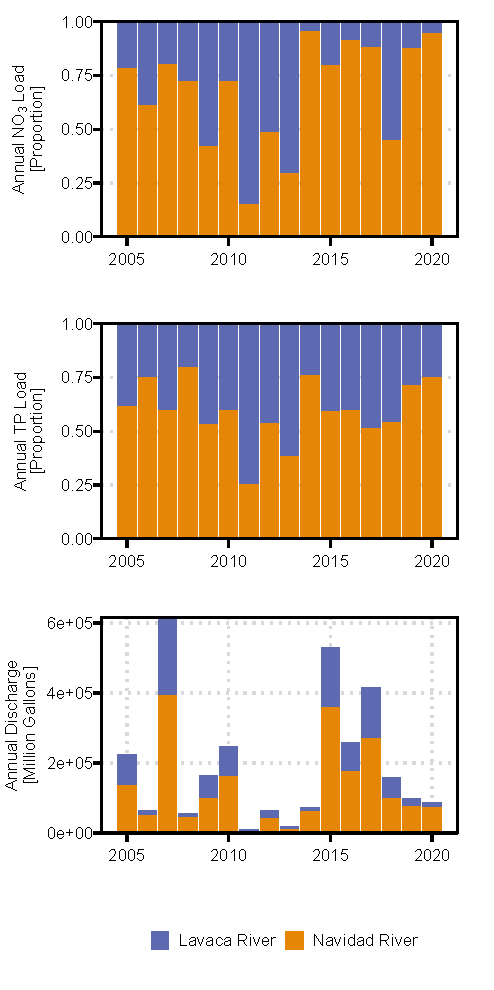
\includegraphics[width=0.5\linewidth,]{Schramm-2023-08-PeerJ_files/figure-latex/fig4} 

}

\caption{Comparison of delivered annual loads and annual discharge at the Lavaca (USGS-08164000) and Navidad (USGS-08164525) Rivers.}\label{fig:fig4}
\end{figure}

\hypertarget{linkages-between-water-quality-and-watershed-flows-and-loads}{%
\subsection*{Linkages Between Water Quality and Watershed Flows and
Loads}\label{linkages-between-water-quality-and-watershed-flows-and-loads}}
\addcontentsline{toc}{subsection}{Linkages Between Water Quality and
Watershed Flows and Loads}

There was no evidence of long-term changes in TP or DO concentrations at
any Lavaca Bay site (Fig.~\ref{fig:fig5}). The upper-bay site
(TCEQ-13563) had evidence of a long-term linear increase in
NO\textsubscript{\emph{X}} while chlorophyll-\emph{a} decreased from
2005 through 2014 (Fig.~\ref{fig:fig5}). NO\textsubscript{\emph{X}}
concentration at the mid-bay site (TCEQ-13383) displayed a periodic
pattern that is indicative of a strong influence from inflow or
precipitation. The temporal GAMs did not provide evidence of long-term
trends in any of the water quality constituents at the lower-bay site
(TCEQ-13384).

\begin{figure}

{\centering 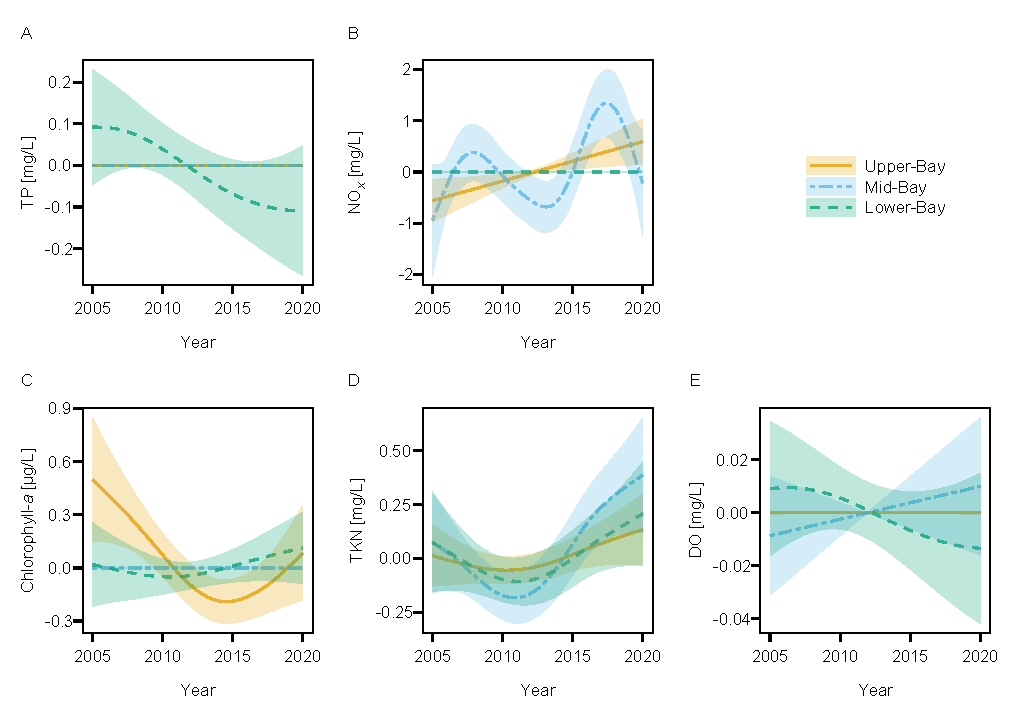
\includegraphics[width=1\linewidth,]{Schramm-2023-08-PeerJ_files/figure-latex/fig5} 

}

\caption{Fitted splines (shaded regions indicate 90\% confidence intervals) from the temporal estuary GAM (Table \ref{tab:table3}) display the marginal smoothed effect of date on TP (A), NO\textit{\textsubscript{X}} (B), chlorophyll-\textit{a} (C), TKN (D), and DO (E) concentrations at each site in Lavaca Bay.}\label{fig:fig5}
\end{figure}

Freshwater inflow provided additional explanation for changes in
NO\textsubscript{x} and chlorophyll-\emph{a} at all of the Lavaca Bay
sites according to AIC\textsubscript{c} and model probability values
(Table~\ref{tab:table4}). Freshwater inflow also explained additional
variation in TP at the upper- and mid-bay sites but not the lower-bay
site. Freshwater inflow did not explain additional variation in TKN
concentrations at any of the sites. The upper- and lower-bay sites saw
improvements in explanation of DO concentration with the inclusion of
inflow.

Inclusion of TP loads provided additional explanation of TP
concentrations at the upper- and mid-bay sites. Inclusion of
NO\textsubscript{3} loads did not provide model explanatory improvements
at any of the sites. The addition of nutrient loads (both TP and
NO\textsubscript{3}) terms did not provide additional explanation for
changes in DO concentrations but did provide model improvement for the
chlorophyll-\emph{a} model at the mid-bay site.

Increases in aggregated freshwater inflow resulted in increases in TP at
the upper- and mid-bay sites and increases in NO\textsubscript{\emph{X}}
and chlorophyll-\emph{a}concentration at all three sites
(Fig.~\ref{fig:fig6}). Linear increases in DO concentration were
observed with increasing flow at the upper- and lower-bay sites. TKN
showed no response to changes in inflow at any of the sites.

Increased TP loads resulted in nearly linear increases of TP
concentration at the upper- and mid-bay sites (Fig.~\ref{fig:fig7}). The
relative effect size appeared much smaller than the effect of freshwater
inflow alone. Increased NO\textsubscript{3} loads did effect
NO\textsubscript{x} concentrations at any site. Linear increases in
chlorophyll-\emph{a} were observed in response to increased TP loads at
the mid-bay site, but not the other sites or in response to
NO\textsubscript{3} loads.

\begin{table}

\caption{\label{tab:table4}Estuary GAM AIC\textsubscript{c} values and associated model probabilities (in parenthesis). Models with the highest probability for each site and water quality parameter combination are bolded and italicized for emphasis.}
\centering
\begin{tabular}[t]{ll>{}l>{}l>{}l}
\toprule
Parameter & Site & Temporal & Inflow & Inflow + Load\\
\midrule
 & Upper-Bay & -145.3 (0.01) & -150 (0.12) & \em{\textbf{-154 (0.87)}}\\

 & Mid-Bay & -152.1 (0.02) & -155.1 (0.07) & \em{\textbf{-160.2 (0.91)}}\\

\multirow{-3}{*}{\raggedright\arraybackslash TP} & Lower-Bay & \em{\textbf{-194.4 (0.39)}} & -194 (0.31) & -194 (0.31)\\
\cmidrule{1-5}
 & Upper-Bay & -175.1 (0.01) & \em{\textbf{-183.8 (0.5)}} & -183.8 (0.5)\\

 & Mid-Bay & -218.9 (0) & \em{\textbf{-241.7 (0.5)}} & -241.7 (0.5)\\

\multirow{-3}{*}{\raggedright\arraybackslash NO\textsubscript{x}} & Lower-Bay & -263.4 (0) & \em{\textbf{-298.1 (0.5)}} & -298.1 (0.5)\\
\cmidrule{1-5}
 & Upper-Bay & 289.5 (0.37) & \em{\textbf{289.5 (0.38)}} & 290.3 (0.25)\\

 & Mid-Bay & 279.7 (0.24) & 279.6 (0.26) & \em{\textbf{278.2 (0.5)}}\\

\multirow{-3}{*}{\raggedright\arraybackslash Chlorophyll-\textit{a}} & Lower-Bay & 268.2 (0.03) & \em{\textbf{262.7 (0.48)}} & 262.7 (0.48)\\
\cmidrule{1-5}
 & Upper-Bay & \em{\textbf{31.1 (0.5)}} & 31.1 (0.5) & -\\

 & Mid-Bay & \em{\textbf{42.2 (0.5)}} & 42.2 (0.5) & -\\

\multirow{-3}{*}{\raggedright\arraybackslash TKN} & Lower-Bay & \em{\textbf{34.3 (0.5)}} & 34.3 (0.5) & -\\
\cmidrule{1-5}
 & Upper-Bay & 138.3 (0.17) & \em{\textbf{136.4 (0.42)}} & 136.4 (0.42)\\

 & Mid-Bay & \em{\textbf{146.4 (0.37)}} & 146.8 (0.29) & 146.5 (0.34)\\

\multirow{-3}{*}{\raggedright\arraybackslash DO} & Lower-Bay & 135.9 (0.04) & \em{\textbf{130.6 (0.48)}} & 130.6 (0.48)\\
\bottomrule
\end{tabular}
\end{table}

\begin{figure}

{\centering 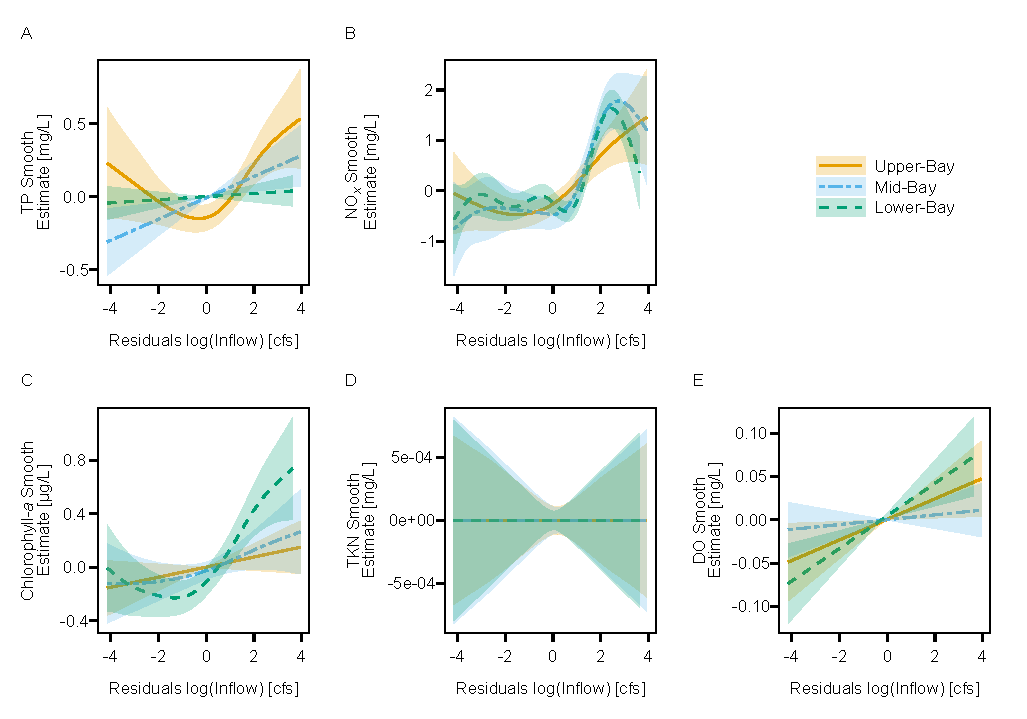
\includegraphics[width=1\linewidth,]{Schramm-2023-08-PeerJ_files/figure-latex/fig6} 

}

\caption{Fitted splines from estuary GAMs display the marginal smoothed effect of freshwater inflow (controlled for season) on TP (A), NO\textit{\textsubscript{X}} (B), chlorophyll-\textit{a} (C), TKN (D), and DO (E) concentrations at each site in Lavaca Bay.}\label{fig:fig6}
\end{figure}

\begin{figure}

{\centering 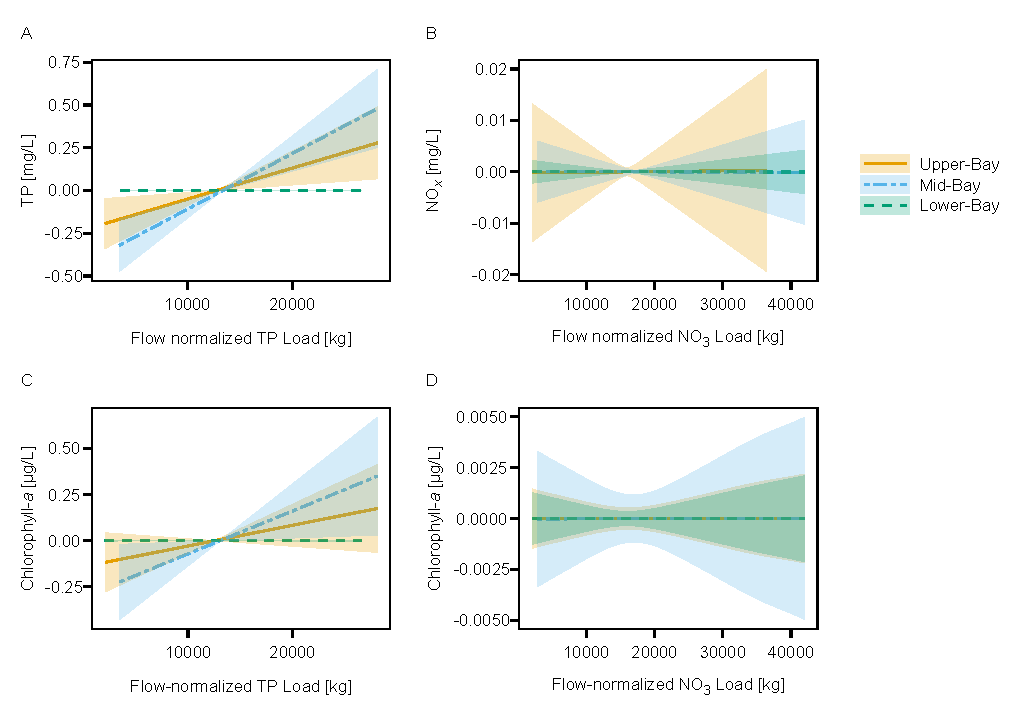
\includegraphics[width=1\linewidth,]{Schramm-2023-08-PeerJ_files/figure-latex/fig7} 

}

\caption{Fitted splines from the nutrient loading GAMs display the marginal smoothed effect of 20-day aggregated TP and NO\textsubscript{3} flow-normalized loads on (A) TP, (B) NO\textsubscript{\textit{X}}, and (C,D) chlorophyll-\textit{a} concentrations at each site in Lavaca Bay.}\label{fig:fig7}
\end{figure}

\hypertarget{discussion}{%
\section*{Discussion}\label{discussion}}
\addcontentsline{toc}{section}{Discussion}

\hypertarget{nutrient-loads}{%
\subsection*{Nutrient Loads}\label{nutrient-loads}}
\addcontentsline{toc}{subsection}{Nutrient Loads}

TP and NO\textsubscript{3} loadings from the Lavaca Bay watershed showed
high inter-annual variability driven primarily by fluctuations in
discharge. Notably, there were no indications of trends in
flow-normalized NO\textsubscript{3} and TP loads in the Navidad River.
In comparison, there was weak evidence of more recent decreases in
flow-normalized NO\textsubscript{3} (but not TP) loads in the Lavaca
River watershed. While the dominant agricultural land uses differ
between the Lavaca (primarily grazed pasture and rangeland) and Navidad
(mix of pasture and row crops) catchments, we did not have a reason to
expect different flow normalized trends between the two systems from
land use alone. Freshwater discharges in the Navidad River are regulated
by the Palmetto Bend Dam forming Lake Texana at the lower extent of the
river. Lentic nitrogen uptake and cycling may have regulating effects
that mask changes in upstream nitrogen loadings. Additional nutrient
data collection in the tributaries of Lake Texana is needed to fully
assess the role of Lake Texana in regulating nutrient delivery to the
Lavaca Bay system. However, these results suggest that there have been
no changes in the NO\textsubscript{3} or TP loading from the Navidad
River system at the Lake Texana discharge point when accounting for
variations in year to year discharge.

The evidence of decreased Lavaca River NO\textsubscript{3} loading,
although weak, is a potential positive sign for water quality managers
working to implement practices that improve water quality in the
freshwater sections of the Lavaca River watershed. Planning and
implementation efforts to increase agricultural producer participation
in water quality protection practices have been ongoing in the watershed
since 2016
\autocite{schrammLavacaRiverWatershed2018,bertholdDirectMailingEducation2021},
however little work has been conducted to directly link these efforts
with water quality outcomes. The decrease in flow-normalized
NO\textsubscript{3} loads could be a reflection of those collective
efforts but the lack of evidence for similar changes in flow-normalized
TP loads provide contrary support. The inconsistent flow-normalized
trends may also reflect some of the weakness of the water quality
dataset that is primarily composed of ambient water quality
measurements. The issues associated with the lack of flow-biased
measurements is further discussed later in this section.

Some prior studies have generated estimates of mean annual TP yields in
the Lavaca River watershed
\autocites[Table~\ref{tab:table5},][]{dunnTrendsNutrientInflows1996,rebichSourcesDeliveryNutrients2011,omaniEstimationSedimentNutrient2014,wise_spatially_2019}.
Although these studies differ in time periods and methodologies, they
provide a sanity check for the reasonableness of the annual estimates
generated in the current study. In a regional assessment of nutrient
loading in river's along the Gulf of Mexico,
\textcite{dunnTrendsNutrientInflows1996} used the LOADEST model to
develop an estimated mean annual yield of 28.9 kg/km\textsuperscript{2}.
LOADEST is a multiple linear regression model that fits log transformed
pollutant concentrations to long term, seasonal, and flow based
predictors and includes methods for bias correction when exponentiating
the response variable. \textcite{rebichSourcesDeliveryNutrients2011} and
\textcite{wise_spatially_2019} used SPARROW to provide a more recent
assessment of regional catchment based loadings to the Gulf of Mexico
(Table~\ref{tab:table5}). SPARROW is a hybrid statistical-process model
with the underlying nutrient load estimation methods based on the
previously described LOADEST
\autocite{schwarzSPARROWSurfaceWaterQuality2006}. The functional form of
the LOADEST regression model is similar to the terms applied in the GAMs
used in the current study. The only study to apply a mechanistic
watershed model (SWAT) to estimate nutrient loadings in the Lavaca River
watershed \textcite{omaniEstimationSedimentNutrient2014} developed
estimated yields (42 kg/km\textsuperscript{2}) similar to the two
SPARROW models. Although direct comparisons are complicated by varying
time periods, the estimates in this study do fall within the range of of
previously developed estimates. To evaluate changes in long-term trends
in discharge might be associated with the nutrient yield estimates
covering different time periods, we fit a GAM relating log-transformed
daily discharges on the Lavaca River to season and time
(Fig.~\ref{fig:fig8}). The long-term trends in discharge indicate
watershed discharges were at or above average from 1972 though the early
and mid-1980s. In comparison watershed discharges since the mid-2000s
are at or below average. It is probable that the lower than average
discharges observed from 2010 through 2021 (Fig.~\ref{fig:fig8}) bias
our estimates downward compared to studies that included higher than
average streamflow periods (1995-2005). Overall, the ranges of estimated
yields among different studies along with the apparent large variability
in streamflow driven loadings (Fig.~\ref{fig:fig3}, Fig. \ref{fig:fig4})
suggest that the current estimates of TP loading are reasonable.

\begin{figure}

{\centering 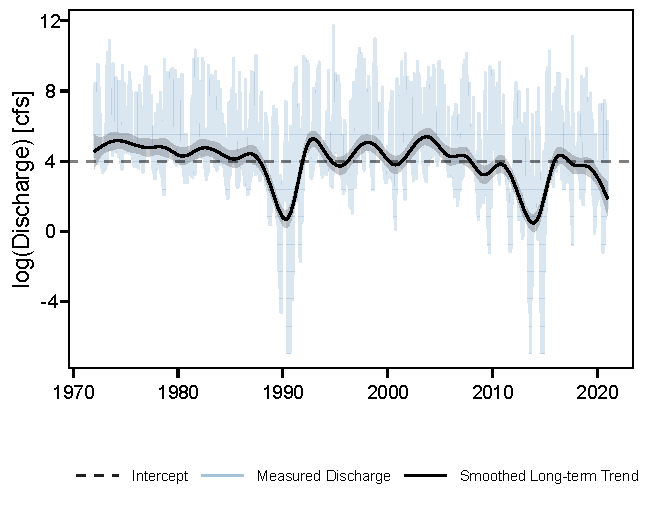
\includegraphics[width=0.7\linewidth,]{Schramm-2023-08-PeerJ_files/figure-latex/fig8} 

}

\caption{Measured daily discharges (log-transformed) and smoothed long-term trends for the Lavaca River form 1972 though 2001.}\label{fig:fig8}
\end{figure}

\begin{table}

\caption{\label{tab:table5}Comparisons of previously published estimates of mean annual TP yield at the Lavaca River site.}
\centering
\begin{tabular}[t]{llll}
\toprule
Reported Yield (kg$\cdot$km\textsuperscript{2}$\cdot$year\textsuperscript{-1}) & Approach & Time Period & Reference\\
\midrule
35.2 (28.8, 43.3)\textsuperscript{a} & GAM & 2005-2020 & This work\\
45.2 & SPARROW & 2000-2014 & \cite{wise_spatially_2019}\\
42 & SWAT & 1977-2005 & \cite{omaniEstimationSedimentNutrient2014}\\
20.81-91.58\textsuperscript{b} & SPARROW & 1980-2002 & \cite{rebichSourcesDeliveryNutrients2011}\\
28.9 & LOADEST & 1972-1993 & \cite{dunnTrendsNutrientInflows1996}\\
\bottomrule
\multicolumn{4}{l}{\rule{0pt}{1em}\textsuperscript{a} Mean of the annual point estimates and the lower and upper 90\% credible intervals.}\\
\multicolumn{4}{l}{\rule{0pt}{1em}\textsuperscript{b} Represents a binned value range from a choropleth map.}\\
\end{tabular}
\end{table}

\hypertarget{estuary-water-quality}{%
\subsection*{Estuary Water Quality}\label{estuary-water-quality}}
\addcontentsline{toc}{subsection}{Estuary Water Quality}

The non-linear estuary water quality trends identified in the current
study differed slightly from previously identified trends
\autocite{bugica_water_2020}. This is not unexpected due to the
different time periods, different methodology, and generally small
slopes identified for most of the significant water quality parameters
in prior work. Both DO and cholorophyll-\emph{a} concentrations at all
three Lavaca Bay sites were stable from 2005 through 2020. This is a
positive outcome in comparison to other Texas estuaries that are facing
larger demands for freshwater diversions, higher population growth, and
more intense agricultural production which have resulted in more direct
signs of eutrophication
\autocite{wetzWaterQualityDynamics2016,bugica_water_2020}. Despite the
stability of DO and cholorophyll-\emph{a}, there are concerning site
specific increases in NO\textsubscript{\emph{X}} and TKN concentration
over the same time period. These trends are especially concerning due to
the nitrogen limitation identified in many Texas estuaries
\autocite{gardnerNitrogenFixationDissimilatory2006,houTransformationFateNitrate2012,doradoUnderstandingInteractionsFreshwater2015,paudelRelationshipSuspendedSolids2019,wetz_exceptionally_2017}
and the relatively low ambient concentrations observed in Lavaca Bay.

The strong positive effect of freshwater inflow on
NO\textsubscript{\emph{X}} and TP concentration are suggestive of
nonpoint watershed sources, consistent with watershed uses and with
other studies relating freshwater inflow with nutrient concentrations in
Lavaca Bay and other estuaries
\autocite{russell_effect_2006,caffreyHighNutrientPulses2007,peierlsNonmonotonicResponsesPhytoplankton2012,palmerImpactsDroughtsLow2015,ciraPhytoplanktonDynamicsLowinflow2021}.
Inflow had a non-linear relationship with NO\textsubscript{x}, with
NO\textsubscript{x} increasing as freshwater inflow transitioned from
low to moderate levels. At higher freshwater inflows, the
NO\textsubscript{x} decreased at the mid- and lower-bay sites, possibly
indicating a flushing effect at higher freshwater inflow. No
relationship between TKN and freshwater inflow was observed at any of
the sites. The results coincide with previous work that suggest
processing of organic loads in the tidal portions of the Lavaca River
reduce transport of nutrients to the lower reaches of Lavaca Bay
\autocite{russell_effect_2006}.

Freshwater inflow also displayed positive effects on
chlorophyll-\emph{a} at each site, with the largest effect at the
lower-bay site. The lower-bay site also showed an attenuation in in
chlorophyll-\emph{a} at the highest freshwater inflow volumes.
Freshwater flushing or increases in turbidity are associated with
limitations or decreases in chlorophyll-\emph{a} in other estuaries
\autocite{peierlsNonmonotonicResponsesPhytoplankton2012,cloernPhytoplanktonPrimaryProduction2014}.
No relationships between inorganic nitrogen and chlorophyll-\emph{a}
were observed. However, a small positive effect between flow-normalized
TP loads and chlorophyll-\emph{a} concentrations were detected at the
mid-bay site. Although, this is not suggestive of a phosphorus
limitation in the Bay, it is supportive of prior work emphasizing the
importance of controlling both nitrogen and phosphorus runoff to protect
water quality \autocite{conleyControllingEutrophicationNitrogen2009}.
Due to the lack of TKN loading information, no assessment between
organic nitrogen loads and chlorophyll-\emph{a} were possible.

Although other studies have identified complex relationships between
estuary nutrient concentrations, nutrient loading and
chlorophyll-\emph{a} concentrations in Texas estuaries
\autocite{ornolfsdottirNutrientPulsingRegulator2004,doradoUnderstandingInteractionsFreshwater2015,ciraPhytoplanktonDynamicsLowinflow2021,tominackVariabilityPhytoplanktonBiomass2022},
this study specifically used flow-adjusted freshwater derived nutrient
loads to parse out contributions from changes in nutrient loadings while
accounting for variations in load due to flow. Loading GAMs indicated no
evidence of changes in flow-normalized TP loads in either river, and no
changes in flow-normalized NO\textsubscript{3} loads in the Navidad
River. The small changes in flow-normalized NO\textsubscript{3} loads in
the Lavaca River are probably masked under most conditions by discharge
from the Navidad River. Given the relatively small variation in
flow-normalized loads, it can be expected that they would contribute
little to the variance in downstream water quality.

There was no evidence that adjusted freshwater inflow and nutrient loads
had effects on DO concentration in Lavaca Bay. The seasonality term in
the temporal GAM models explained a substantial amount of DO variation
at all of the sites. Responses of estuary metabolic processes and
resulting DO concentrations can be quite complicated and often locally
specific \autocite{caffreyFactorsControllingNet2004}. While the lack of
total nitrogen or TKN loading data hinders interpretation, the large
seasonal effect on DO concentration indicates physical factors (such as
temperature, wind, and turbidity) play an important role and should be
included in future models. Prior work suggests that Lavaca Bay may not
be limited by nutrients alone, with high turbidity or nutrient
processing in upper portions of the Bay or intertidal river limiting
production \autocite{russell_effect_2006}. Finally, it is reasonable to
assume that fluctuations in DO may not occur immediately in response to
nutrient pulses or freshwater inflow. Work has shown that many water
quality parameters may have lagged effects lasting days or even months
following storms and large discharge events
\autocite{mooneyWatershedExportEvents2012a,wetzExtremeFutureEstuaries2013,bukaveckasInfluenceStormEvents2020,walkerTimescalesMagnitudeWater2021}.
However, this study only evaluated responses to loading and inflows
occurring the day of water quality observations.

Overall, this study suggests that DO and chlorophyll-\emph{a}
concentrations have been relatively stable in Lavaca Bay. Site-specific
increases in TKN and NO\textsubscript{\emph{X}} concentrations are a
cause of concern for increasing risks of eutrophication within Lavaca
Bay which might be currently attenuated by changes in freshwater flow,
turbidity, and other physical processes. While loading models indicate
that there are large annual fluctuations in NO\textsubscript{3} loads,
these changes have been largely driven environmental conditions (changes
in runoff and river discharge). These models also provide evidence that
estuary NO\textsubscript{\emph{X}} and TP concentrations are strongly
driven by freshwater inflow and to a lesser extent fluctuation in
flow-normalized riverine loadings. Site-specific changes in the
relationships between freshwater inflow and responses in both
chlorophyll-\emph{a} and NO\textsubscript{x} concentrations are
indicative of nutrient processing and or tidal flushing effects moving
from the river discharge point to the mouth of Lavaca Bay. This study
does not completely explain site specific increases in
NO\textsubscript{\emph{X}} and TKN concentrations in Lavaca Bay. The
freshwater study sites did not quantify nutrient loadings from tidal
contribution areas or ungauaged watersheds. Nutrient contributions from
wastewater facility discharges, septic systems, and stormwater could be
considerable contributors to nutrient loadings in Lavaca Bay since they
are not processed by a tidal river reach prior to entering the Bay. The
Garcitas-Arenosa Creek, Placedo Creek, and Cox Bay subwatersheds are
currently undersampled but compose approximately 27\% of the watershed
area. The contribution of nutrient loadings from these undersampled
areas is unknown.

\hypertarget{future-management-and-research-needs}{%
\subsection*{Future Management and Research
Needs}\label{future-management-and-research-needs}}
\addcontentsline{toc}{subsection}{Future Management and Research Needs}

The GAM approach proved useful for both estimating loads and assessing
downstream responses in water quality. Although we did not compare other
models, it is likely similar estimates of loadings would be obtained by
methods such as LOADEST, WRTDS, or SPARROW given the functionally
similar dependent variable structures. The underlying weakness in the
estimates of loading in the current study is the reliance on ambient
water quality data used for statewide water quality assessments.
Cross-validation of the nutrient loading models highlights that
predictions are prone to high bias, owing to the lack of targeted storm
or flow biased measurements. The high biases are indicative that subsets
of values were unable to capture the functional relationships with the
flow based dependent variables. It was beyond the scope of the current
study to evaluate the subsets of cross-validation data and scores.
However, the cross-validation procedure is indicative that more robust
sampling is needed. Supplementary flow-biased monitoring targeting
storm- or high-flow conditions is critical to improve model performance
and strength of evidence produced by these models
\autocite{horowitzEvaluationSedimentRating2003,snelderEstimationCatchmentNutrient2017}.
Although there is existing work on the samples sizes and sample design
required for reliable performance of both LOADEST
\autocite{parkUsePollutantLoad2014} and WRTDS
\autocite{kumarValueIntensiveSampling2019} models, similar work does not
appear to have been extended to water quality applications of GAMs.

Due to the concerning increases in eutrophication associated parameters
in Lavaca Bay and other Texas estuaries \autocite{bugica_water_2020},
and the desire to quantify linkages between environmental outcomes and
on the ground management actions \autocite{schrammTotalMaximumDaily2022}
there is a strong need for reliable estimates of pollutant loadings and
responses along the Texas coast. Within Texas, statewide water quality
monitoring programs have focused on collection of ambient condition
data. A framework for establishing pollutant load monitoring programs
across catchments that explicitly incorporate flow biased data is needed
for assessing nutrient loading and estuary health along the Texas coast.

Additional efforts focused on identifying relevant effect sizes,
sampling designs, and funding mechanisms that can support long term
efforts are also needed to adequately design such a framework. Large
long-term monitoring programs in and around the Chesapeake Bay, San
Francisco Bay, and along the Mississippi River have proven extremely
effective at informing management actions and tracking progress towards
long-term pollutant reduction goals. Similar coordinated efforts across
Texas coastal watersheds would prove useful for resource management
efforts intended to protect the biological and water quality integrity
of Texas's estuaries.

\hypertarget{conclusions}{%
\section*{Conclusions}\label{conclusions}}
\addcontentsline{toc}{section}{Conclusions}

The primary purpose of this study was to provide estimates of watershed
nutrient loadings and assess water quality responses to changes in
nutrient loads. GAMs provided reliable estimates of watershed
NO\textsubscript{3} and TP loads. However, additional flow-biased data
collection efforts are needed to decrease the prediction variance and
improve accuracy at critical high-flow loading events. While some
ongoing projects will fill data gaps for total nitrogen and TKN loading,
additional efforts are needed to coordinate data collection efforts
specifically for load estimation across Texas estuaries. Despite these
data gaps, this study identified high annual fluctuations in nutrient
loads driven primarily by discharge. No evidence was identified to
indicate that on the ground management had changed nutrient loading in
the Navidad River subwatershed. There was weak evidence for recent
reductions in flow-normalized NO\textsubscript{3} loading in the Lavaca
River subwatershed although the results are at odds with flow-normalized
trends in TP loads.

This study, consistent with others along the Texas coast, found strong
effects of freshwater flow on nutrient and chlorophyll-\emph{a}
concentrations. DO concentrations, dominated by seasonal effects, did
not show strong direct responses to freshwater flow. Small variances in
flow-adjusted nutrient loads indicate that (1) there have been limited
changes in non-point sources of nutrients and (2) that there is not
strong evidence that those small changes have had extensive effects on
chlorophyll-\emph{a} or dissolved oxygen in Lavaca Bay. Although this
study did not identify changes in DO or chlorophyll-\emph{a}
concentrations in Lavaca Bay, site specific increases in
NO\textsubscript{\emph{X}} and TKN are a cause for water quality
concern. The study provides a baseline assessment for future water
quality management activities in the watershed. In order to effectively
track and link improvements or degradation of water quality conditions
in Lavaca Bay and other coastal Texas watersheds with on the ground
efforts, more robust sampling networks are needed to improve spatial
coverage of undersampled areas and explicitly incorporate flow-biased
sampling.

\hypertarget{acknowledgements}{%
\section*{Acknowledgements}\label{acknowledgements}}
\addcontentsline{toc}{section}{Acknowledgements}

The author thanks Stephanie deVilleneuve for comments on an early draft
and members of the Coastal Nutrient Input Repository project committee
for supporting project development and their valuable input. The views
expressed herein are those of the author(s) and do not necessarily
reflect the views of NOAA, the U.S. Department of Commerce, or any of
their subagencies.

\printbibliography



\end{document}
